\subsection{Trajectoires}
 \begin{frame}[c]
\frametitle{Trajectoires}
   \begin{block}{Trajectoire}
     Une succession de directions
   \end{block}
  \begin{columns}
    \begin{column}[l]{5cm}
      \begin{figure}[!h]
        \begin{center}
          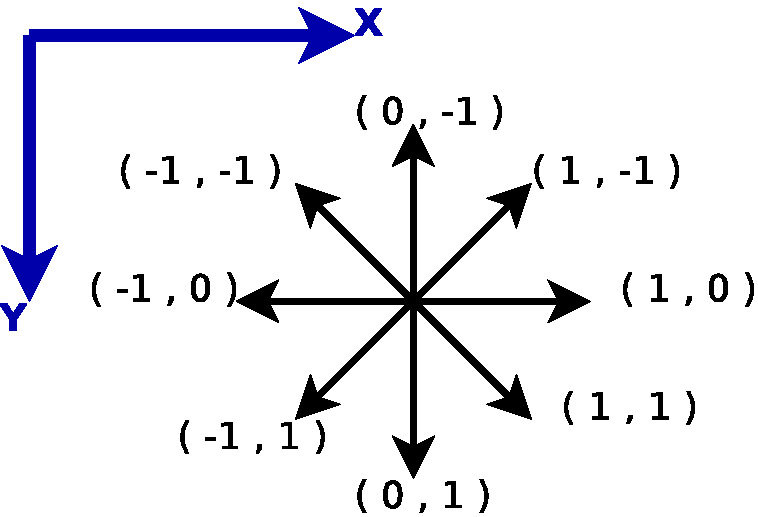
\includegraphics[scale=0.35]{./images/direction.pdf}
        \end{center}
        \caption{Direction}
      \end{figure}
    \end{column}
    \begin{column}[r]{5cm}
      \begin{figure}[!h]
        \begin{center}
          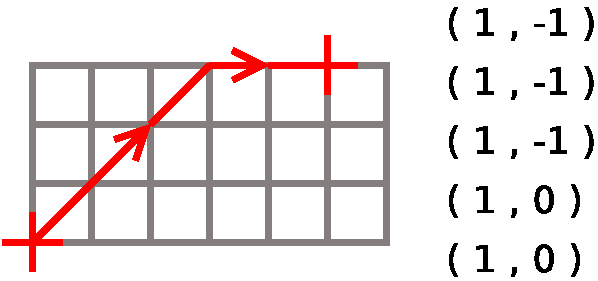
\includegraphics[scale=0.35]{./images/constructionTrajectoire.pdf}
        \end{center}
        \caption{Trajectoire}
      \end{figure}
    \end{column}
  \end{columns}
\end{frame}

\subsection{Collisions}
 \begin{frame}[c]
\frametitle{Collisions}
   \begin{block}{Objets à prendre en compte}
     \begin{itemize}
     \item Bateaux
     \item Berges de la carte
     \item Bords de la carte
     \end{itemize}
   \end{block}
         \begin{figure}[!h]
    \begin{center}
      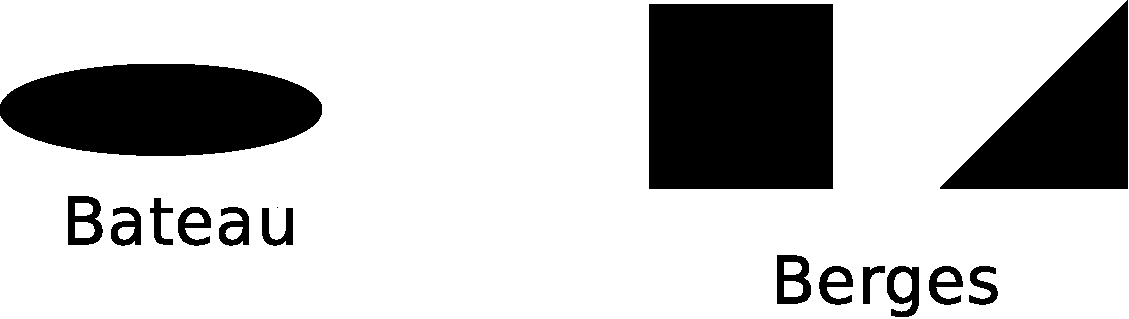
\includegraphics[scale=0.3]{./images/shape.pdf}
    \end{center}
    \caption{Les types de shape}
  \end{figure}
 \end{frame}
